\documentclass{article}

\usepackage{fullpage}
\usepackage{textcomp}
\usepackage{graphicx}

\usepackage{fancyhdr}
\pagestyle{fancy}
\renewcommand{\headrulewidth}{0pt}
\cfoot{\sc Page \thepage\ of \pageref{end}}

\begin{document}

{\large \noindent{}University of Toronto at Scarborough\\
\textbf{CSC A67/MAT A67 - Discrete Mathematics, Fall 2015}}

\section*{\huge Exercise \#5: Logic}

{\large Due: November 6, 2015 at 11:59 p.m.\\
This exercise is worth 3\% of your final grade.}\\[1em]
\textbf{Warning:} Your electronic submission on MarkUs affirms that this exercise is your own work and no
one else's, and is in accordance with the University of Toronto Code of Behaviour on Academic Matters,
the Code of Student Conduct, and the guidelines for avoiding plagiarism in CSC A67/MAT A67.\\[1ex]
This exercise is due by 11:59 p.m. November 6. Late exercises will not be accepted.\\[1ex]
\renewcommand{\labelenumi}{\arabic{enumi}.}
\renewcommand{\labelenumii}{(\alph{enumii})}
\begin{enumerate}
\item If\marginpar{[3]} $k$: ``A bell has been rung", $m$: ``There is meat in the room", and $n$: ``The dogs are salivating",\\
which of the following statements are equivalent to $\neg n\to\neg(m\vee k)$?
	\renewcommand{\labelenumii}{\roman{enumii})}\begin{enumerate}
	\item $\neg n\to\neg m\vee k$
	\item ``If the dogs are not salivating, then there is no meat in the room, or a bell has not been rung."
	\item ``If the dogs are not salivating, then there is no meat in the room and a bell has not been rung."
	\item $n\to (m\vee k)$
	\item $\neg n\to \neg m\vee\neg k$
	\item $\neg n\to \neg m\wedge\neg k$
	\item ``If the dogs are not salivating, then a bell has not been rung, nor is there meat in the room."
	\item $n\vee\neg m\wedge\neg k$
	\item $\neg(m\vee k)\vee n$
	\item ``There is no meat in the room, nor has a bell been rung, if the dogs are not salivating."
	\item ``A bell has not been rung, or there is no meat in the room, if the dogs are not salivating."
	\item ``If a bell has not been rung and there is no meat in the room, then the dogs are not salivating."
	\item ``For the dogs to be salivating, it is sufficent and necessary that a bell has been rung and that there is meat in the room."
	\item $\neg (m\vee k)\to\neg n$
	\item ``For the dogs to be salivating, it is necessary that a bell has been rung and that there is meat in the room."
	\item ``If the dogs are salivating, then a bell has been rung or there is meat in the room."
	\item $n\to m\wedge k$
	\item $\neg n\to m\wedge k$
	\item $n\vee\neg(m\vee k)$
	\item $\neg(m\vee k)\to\neg(\neg n)$
	\end{enumerate}\pagebreak
\item Construct\marginpar{[8]} truth tables for the following statements:
	\renewcommand{\labelenumii}{(\alph{enumii})}\begin{enumerate}
	\item $a\vee b\to\neg b$
	\item $a\wedge b\wedge c$
	\item $\neg\neg a\vee a$
	\item $a\vee b\to a\vee b$
	\end{enumerate}
\item Shade\marginpar{[8]} the regions of a Venn diagram where each of the following statements is true:
	\begin{enumerate}
	\item $\neg p\to q$
	\item $p\leftrightarrow q\vee\neg q$
	\item $\neg p\vee \neg q\wedge p$
	\item $(p\wedge q)\vee(r\wedge q)$
	\end{enumerate}
\item \begin{enumerate}
	\item Negate\marginpar{[4]} the statement ``Sarah has a spaceship and has three fingers and is from Venus" and convert it to formal logic.
	\item Simplify the statement from \textbf{(a)} as much as possible using equivalence rules.
	\end{enumerate}
\item Using\marginpar{[3]} the statements\\
	\begin{tabular}{p{0.47\textwidth}p{0.5\textwidth}}
	\begin{description}
	\item[A:] ``Your vehicle has a District No. 64 permit"
	\item[B:] ``It is between 8am and 9am"
	\item[C:] ``It is a school day (Monday to Friday)"
	\item[D:] ``You have been parked for less than 2 hours during legal hours"
	\item[E:] ``It is between 8am and 6pm"
	\item[F:] ``You have been parked for less than 5 minutes during legal hours"
	\item[G:] ``It is Monday"
	\item[H:] ``You are left of the sign"
	\item[I:] ``It is between 1:30pm and 4pm"
	\item[J:] ``It is between 9am and 10am"
	\item[K:] ``It is after 4pm"
	\item[L:] ``It is after 1pm"
	\end{description}
	create a formal logic statement that is true any time you are allowed to park near the following parking signs, and false any time it is illegal to park there:&
	\begin{center}
	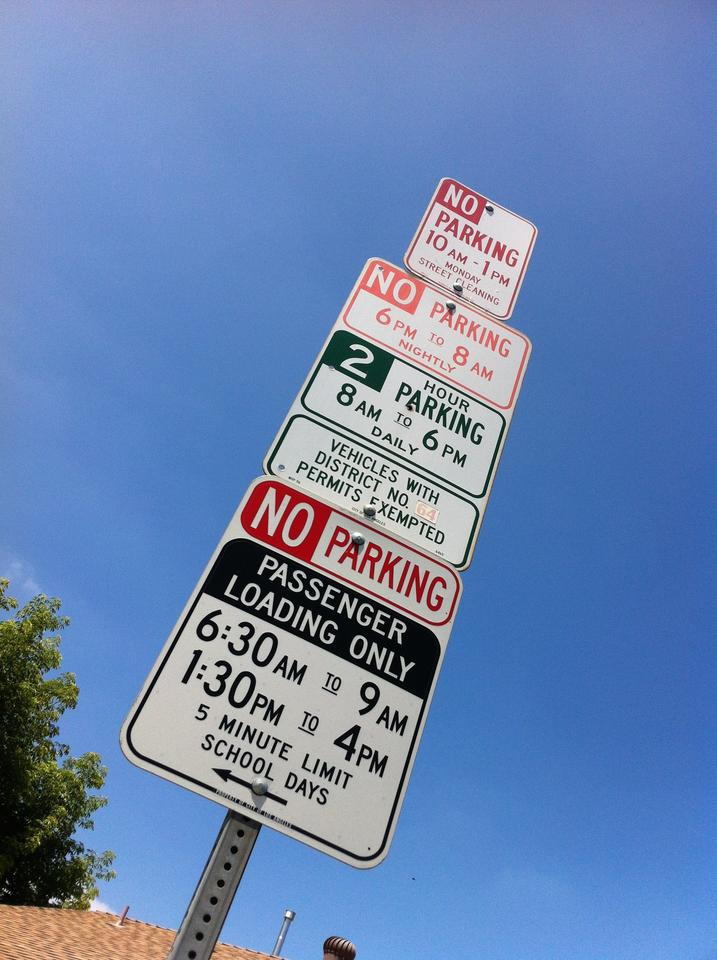
\includegraphics[width=0.4\textwidth,clip,trim=5cm 5cm 5cm 6cm]{Formal-Logic-Exercise-parkingSigns.JPG}
	\end{center}
	\end{tabular}
\end{enumerate}
\hrulefill\\
\noindent[Total: 26 marks]\label{end}

\end{document}